SSM是一个非常广泛的概念,可以认为带有隐状态的循序计算都是SSM模型。
他的思想和和RNN,CNN,Attention这样的神经网络完全不同,背后的想法是让把序列看做是对一个动态系统的离散采样,SSM模型通过微分方程组来建模动态系统状态随时间的变化。

\subsection{一个朴素的直觉解释}

我们首先通过一个全标量计算模型,建立起对state-space model的直觉理解。

\begin{tcolorbox}[colbacktitle=grey!10!white,colback=yellow!3,title={\textbf{\textcolor{grey}{用微分方程组建模动态系统,一个极简例子}}}]
这个\href{https://www.youtube.com/watch?v=8Q_tqwpTpVU}{video}(对应的\href{https://github.com/hkproj/mamba-notes/tree/main}{slides})里speaker举了一个具体的例子来解释用微分方程组建模一个动态系统。
假设我们有一群兔子,每只小兔子在$t$时刻会生$\lambda$只小兔子,$\lambda$是一个固定的常数。
令$b(t)$表示$t$时刻兔子种群一共有多少只兔子,$\frac{db}{dt}$表示$t$时刻兔子种群数目变化的速率,于是有:

$$\frac{db}{dt}=\lambda b(t)$$

已知$t=0$时刻种群有5只兔子,即:$b(t)=5$。我们希望求解出$b(t)$的方程使得对任意$t$,上式都成立,来告诉我们任意时刻,例如$t=100$,种群有多少只兔子。
\end{tcolorbox}

连续时间系统线性SSM模型(continuous-time linear/latent state-space model)将输入信号$x(t)$通过一个隐状态$h(t)$映射到输出信号$y(t)$。

\begin{align}
    h'(t) &= \mathbf{A}h(t) + \mathbf{B}x(t) \label{eq:ssm1}\\
    y(t) &=\mathbf{C}h(t) + \mathbf{D}x(t) \label{eq:ssm2}
\end{align}

\eqref{eq:ssm1}和\eqref{eq:ssm2}已经规定了微分方程组的具体形式,参数化为$\mathbf{A}$,$\mathbf{B}$,$\mathbf{C}$和$\mathbf{D}$。
这样一组微分方程可以用来建模一个动态系统其状态随时间的改变。
求解目标是求解出以上微分方程的具体形式,使得给定系统在0时刻的初始状态,能够计算得到这个动态系统在任意时刻的状态。

为了求解上面这个微分方程组,我们需要找到$h(t)$的具体形式令\eqref{eq:ssm1}等号左右两边相当。
通常情况下找到$h(t)$的解析解是困难的。因此,我们降低要求,\textcolor{tomato}{考虑找到$h(0)$,$h(1)$,$h(2)$,etc.这样一个离散化的序列,用来逼近我们要研究的动态系其状态如何随时间改变}。
因此,我们将寻找$h(t)$转化为对时间进行离散化采样,$k$是采样编号,寻找一个离散化序列$h(t_k) = h(k \triangle)$使以上微分方程系统近似地成立。其中,$\triangle$是step size。

根据导数的定义,我们有:$h'(t) = \lim_{\triangle \rightarrow 0}\frac{h(t+\triangle)-h(t)}{\triangle}$,当step size$\triangle$足够小的时候,我们可以省略极限符号:
$$h(t + \triangle) \approxeq \triangle h'(t) + h(t)$$

将\eqref{eq:ssm1}带入,可得:

\begin{align}
    h(t+\triangle) & \approxeq \triangle \left( \mathbf{A}h(t) + \mathbf{B}x(t)\right) + h(t) \nonumber \\
    &=\triangle \mathbf{A} h(t) + \triangle \mathbf{B}x(t)+h(t) \nonumber \\
    &=\left(\mathbf{I} +\triangle A\right)h(t) + \triangle \mathbf{B} x(t) \nonumber \\
    &\triangleq \bar{\mathbf{A}}h(t) + \bar{\mathbf{B}}x(t) \label{eq:ssm3}
\end{align}

式\eqref{eq:ssm3}是SSM的离散化形式。

\subsection{SSM}

机器学习任务中隐状态均为高维,从上一节的标量形式进一步推广到高维可以参看s4\cite{gu2021efficiently}的论文,这里我们仅关注需要知道的最基本事实。
一个SSM模型的求解需要经过离散化(Zero-Order-Hold(ZOH)或者Bilinear方法),
离散化形式的SSM由以下两个公式表示,其中$\vec{x}$是状态,$\vec{u}$是输入信号,$\vec{y}$是输出信号,

\begin{align}
  \vec{h}_k &= \bar{\mathbf{A}}\vec{x}_{k-1} + \bar{\mathbf{B}}\vec{u}_k \label{eq:ssm4}\\
  \vec{y}_k &= \bar{\mathbf{C}}\vec{x}_k + \bar{\mathbf{D}}\vec{u}_k 
\end{align}

离散化方法会进一步给出$\bar{\mathbf{A}}$,$\bar{\mathbf{B}}$和$\bar{\mathbf{C}}$矩阵的进一步形式。

\textcolor{red}{为了让离散化操作能快速地完成计算,会对矩阵$\mathbf{A}$的形式有所约束,例如为了让矩阵的幂运算快速实现,要求$\mathbf{A}$是一个对角矩阵}。

在预测时候和RNN等价,SSM参数化形式为一组用微分方程组描述的,带隐状态的连续时间系统。通过恰当的离散化方法,能够被转换成CNN或RNN计算。

预测时SSM和RNN计算等价,但是SSM这一类模型的设计来源于不同的理论框架,在训练时有可能带来不同的特性。

\subsection{SSM和RNN的不同之处}

DeepMind的LRU\cite{orvieto2023resurrecting}也讨论了SSM和RNN的不同。

\begin{enumerate}
\item SSM模型离散化之后根据定义\textcolor{red}{在时间维度上是线性的}。也就是说,SSM by definition就是一个linear RNN,在训练的时候适用于以parallel scan模型并行地进行计算;
\item 尽管式\eqref{eq:ssm4}是一个RNN,但是其中$\mathbf{A}$和$\mathbf{B}$有更强的参数化要求。例如,ZOH离散化方法会给出:$\bar{\mathbf{A}}=\exp\left(\triangle \mathbf{A}\right)$,
$\bar{\mathbf{B}}=\left(\bar{\mathbf{A}} -\mathbf{I}\right)\mathbf{A}^{-1} \mathbf{B}$,$\bar{\mathbf{C}}=\mathbf{C}$,
$\bar{\mathbf{D}}=\mathbf{D}$。
\item SSM的初始化非常特殊。recurrent形式的全展开涉及到矩阵的幂运算。为了高效计算矩阵的幂,会要求$\mathbf{A}$是对角矩阵。然而无法总是在实数域将$\mathbf{A}$对角化,但是几乎所有矩阵都能在复数域上对角化,于是SSM将运算放在了复数域,
\footnote{最新的研究通过新的技术放松对这一点的要求}{SSM需要特殊设计的初始化计算}。
\end{enumerate}

\subsection{典型代表}

\subsubsection{S4(\textcolor{blue}{S}tructured \textcolor{blue}{S}tate \textcolor{blue}{S}pace \textcolor{blue}{S}equence models)\cite{gu2021efficiently}}

S4的第一个$S$代表了 "structured"。具体是指:为了SSM能够高效地并行训练,会对矩阵$A$的结构带来一定的约束,目前使用最多的一种约束是要求$A$是一个对角矩阵。

\subsubsection{S5\cite{smith2022simplified}}

\newpage
\subsubsection{Mamba(S6)\cite{gu2023mamba}}

受Transformer整体架构的影响,目前sequence processing模型都是通过反复堆叠一个同构的sequence processing block构成。
这样一个sequence processing block一般由归一化层, token mixer,residual connection三个设计要素构成。
mamba中的norm都用RMSnorm。

\begin{figure}[h]
  \centering
  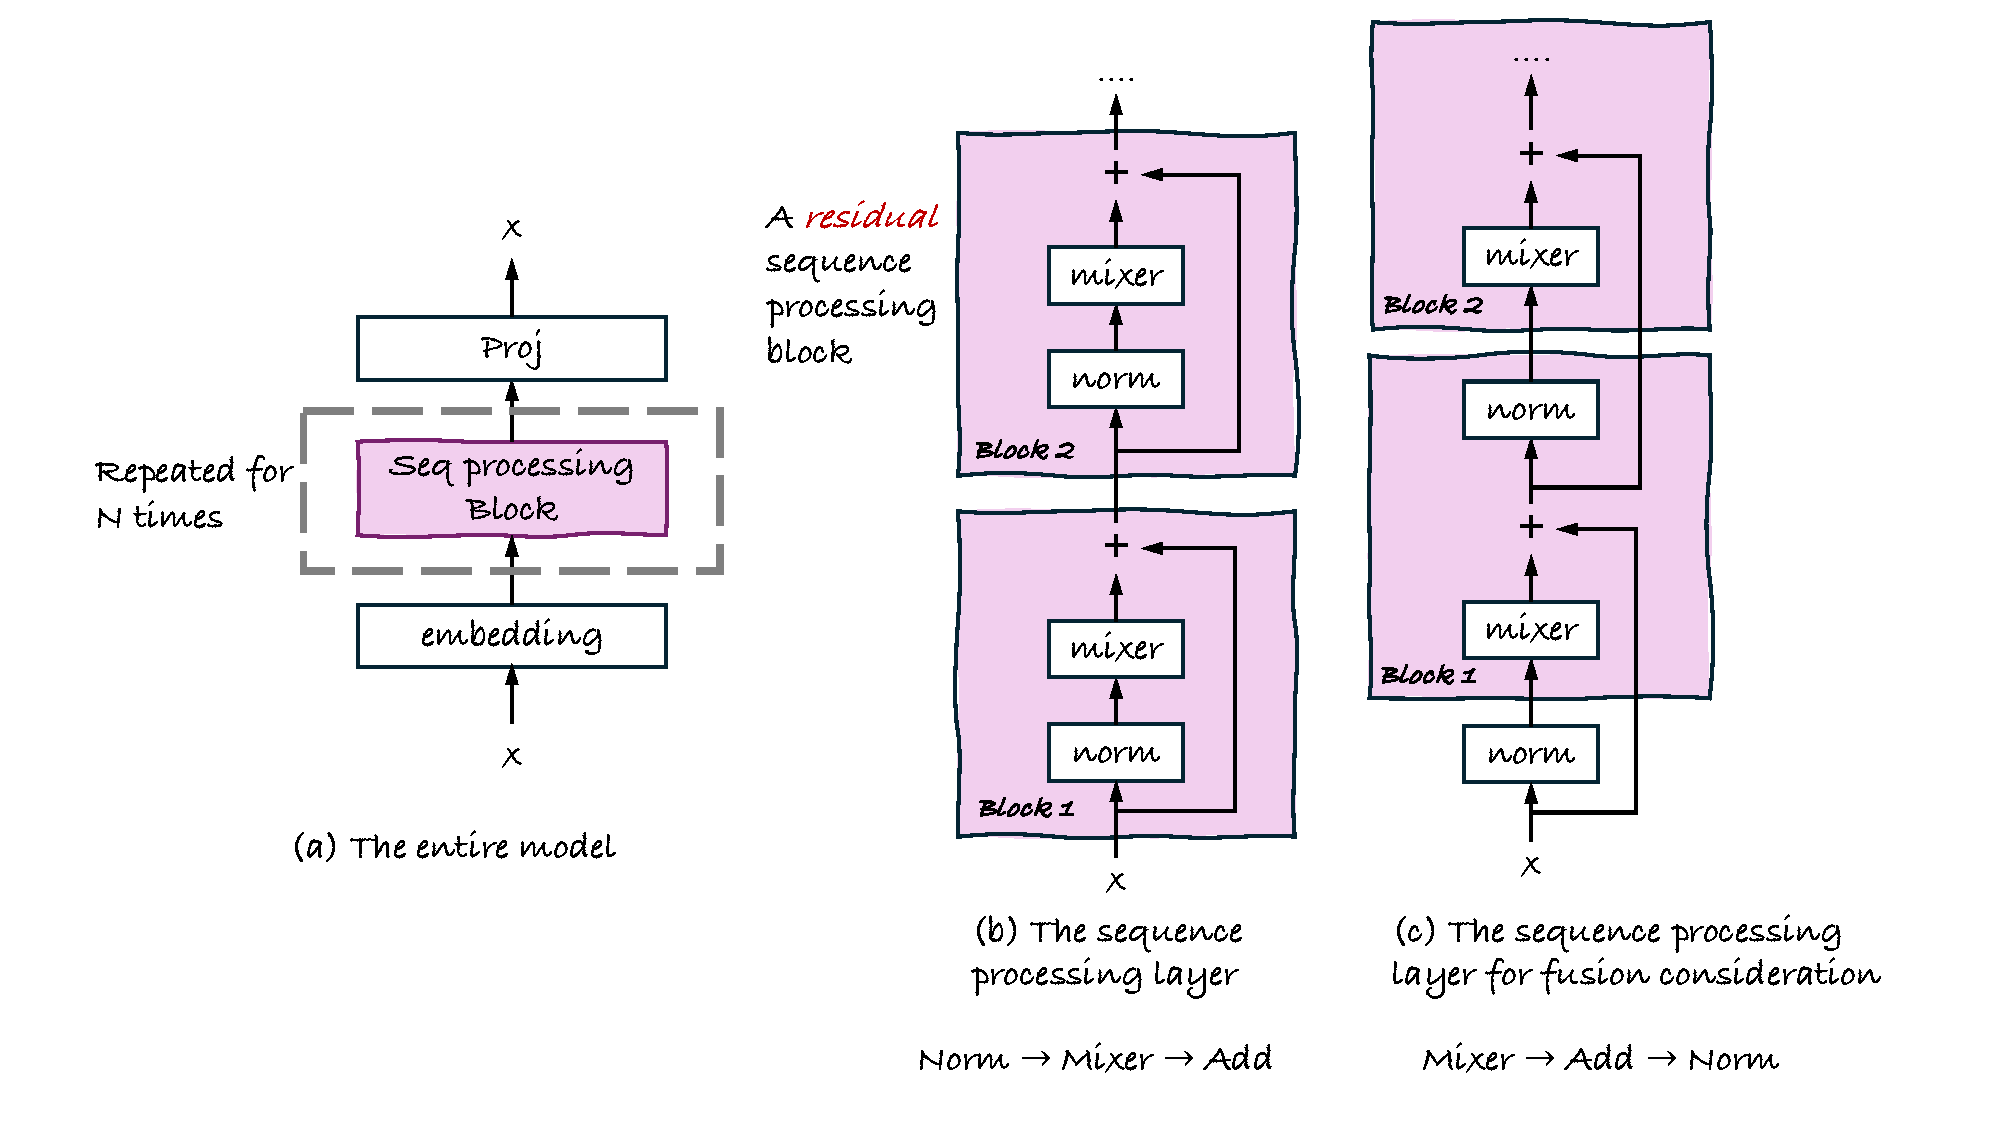
\includegraphics[width=0.85\textwidth]{figures/mamba-model.pdf}
  \caption{mamba模型的整体结构}\label{fig:mamba-model}
\end{figure}

图\ref{fig:mamba-model}(b)的Norm $\rightarrow$ Mixer $\rightarrow$ Add串block的方式更符合设计直觉。
图\ref{fig:mamba-model}(a)的Mixer$\rightarrow$ Add $\rightarrow$ Norm串block的方式更容易在现有PyTorch接口下将Add和Norm进行fuse。

\begin{figure}[h]
  \centering
  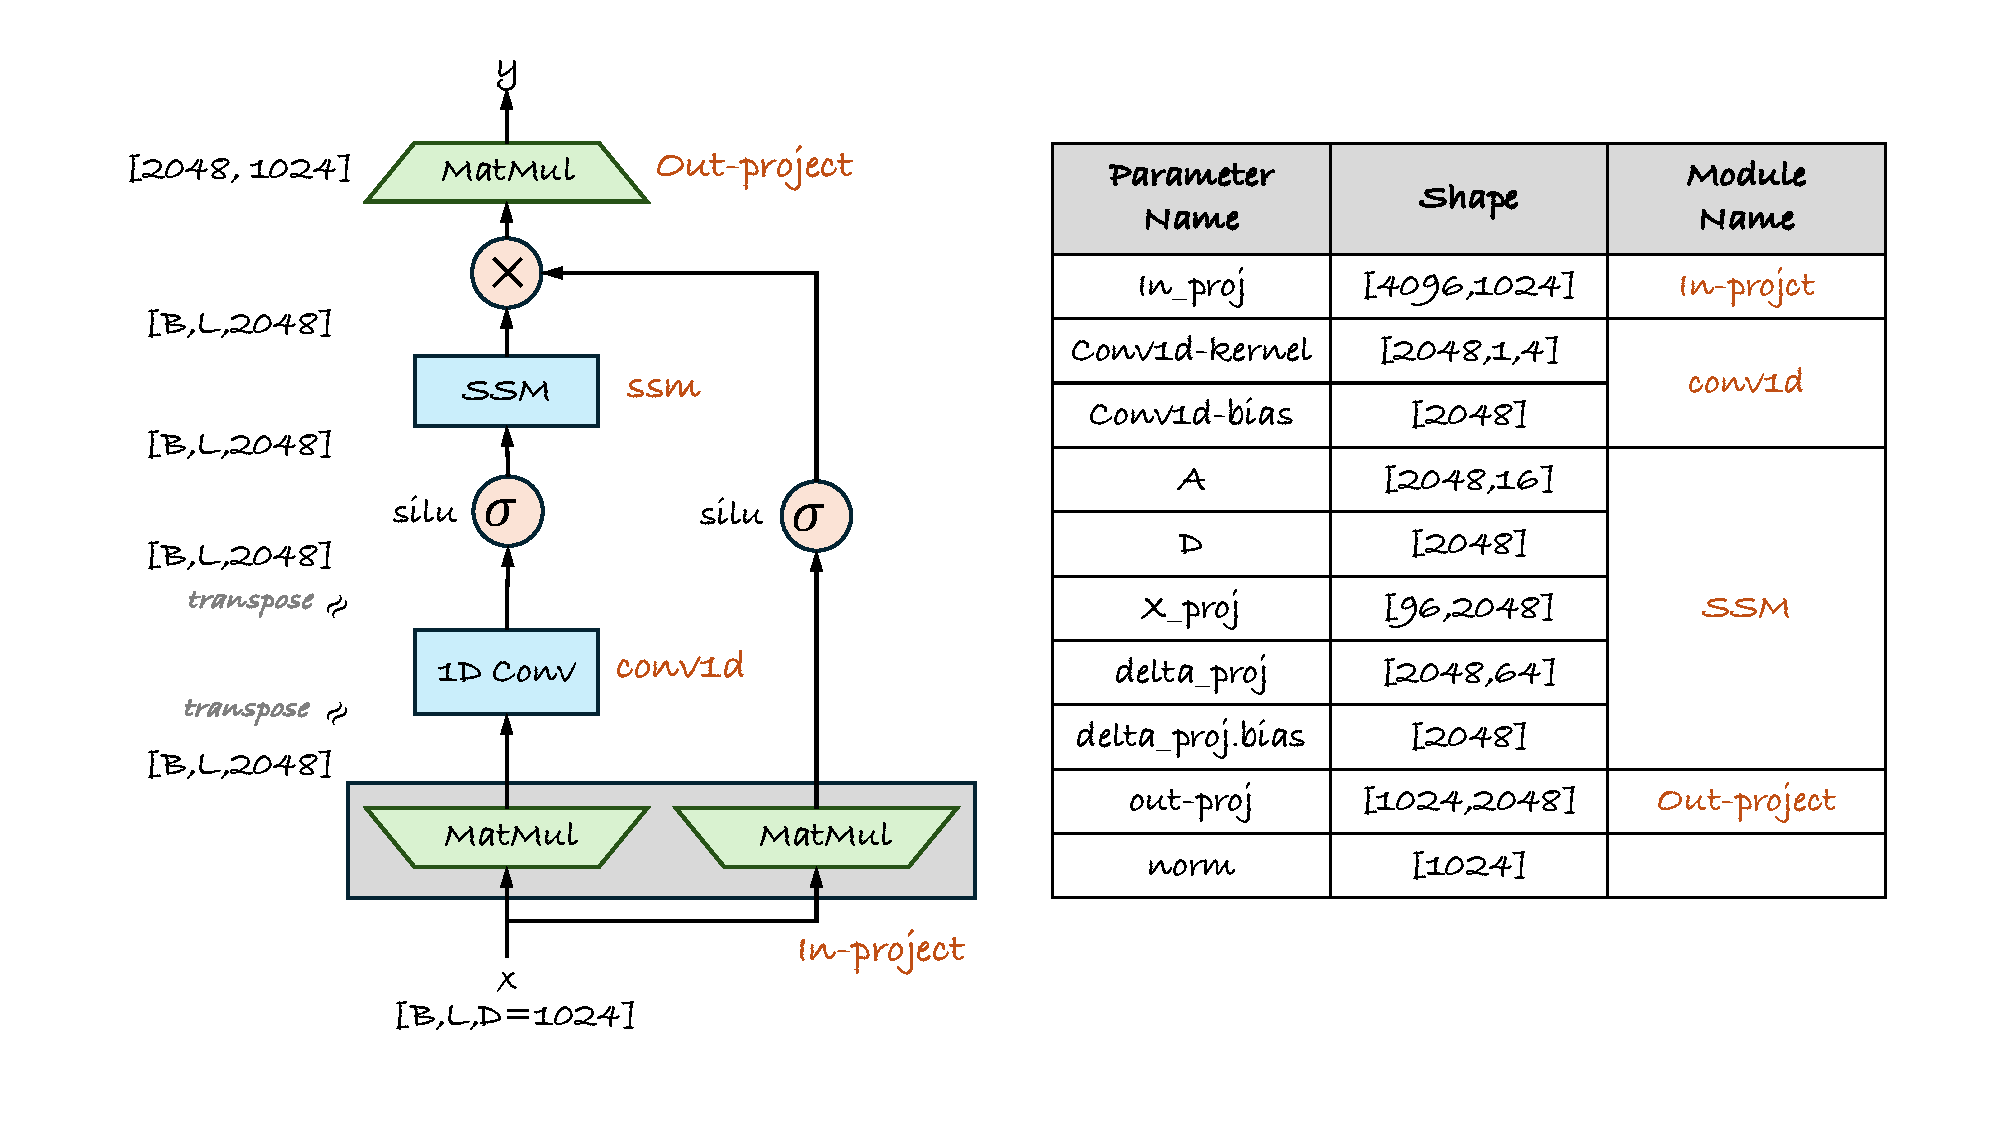
\includegraphics[width=0.9\textwidth]{figures/mamba-mixer.pdf}
  \caption{mamba block作为图\ref{fig:mamba-model}中mixer的细节及可学习参数}\label{fig:mamba-mixer}
\end{figure}

Mamba block是图\ref{fig:mamba-model}中mixer。
Mamba-370m模型里面mamba block堆叠$48$次,输入序列$X$的形状$[B,L,D]$,$D=1024$。

图\ref{fig:mamba-mixer}中SSM部分计算公式如下,其中$u(t)$是整个sequence batch,形状为$[B,L,2048]$,$x(t)$是SSM内部的状态:

\begin{equation}
y(t) = \text{SSM}(u(t)) \label{eq:ssm-0}
\end{equation}

\begin{figure}[h]
  \centering
  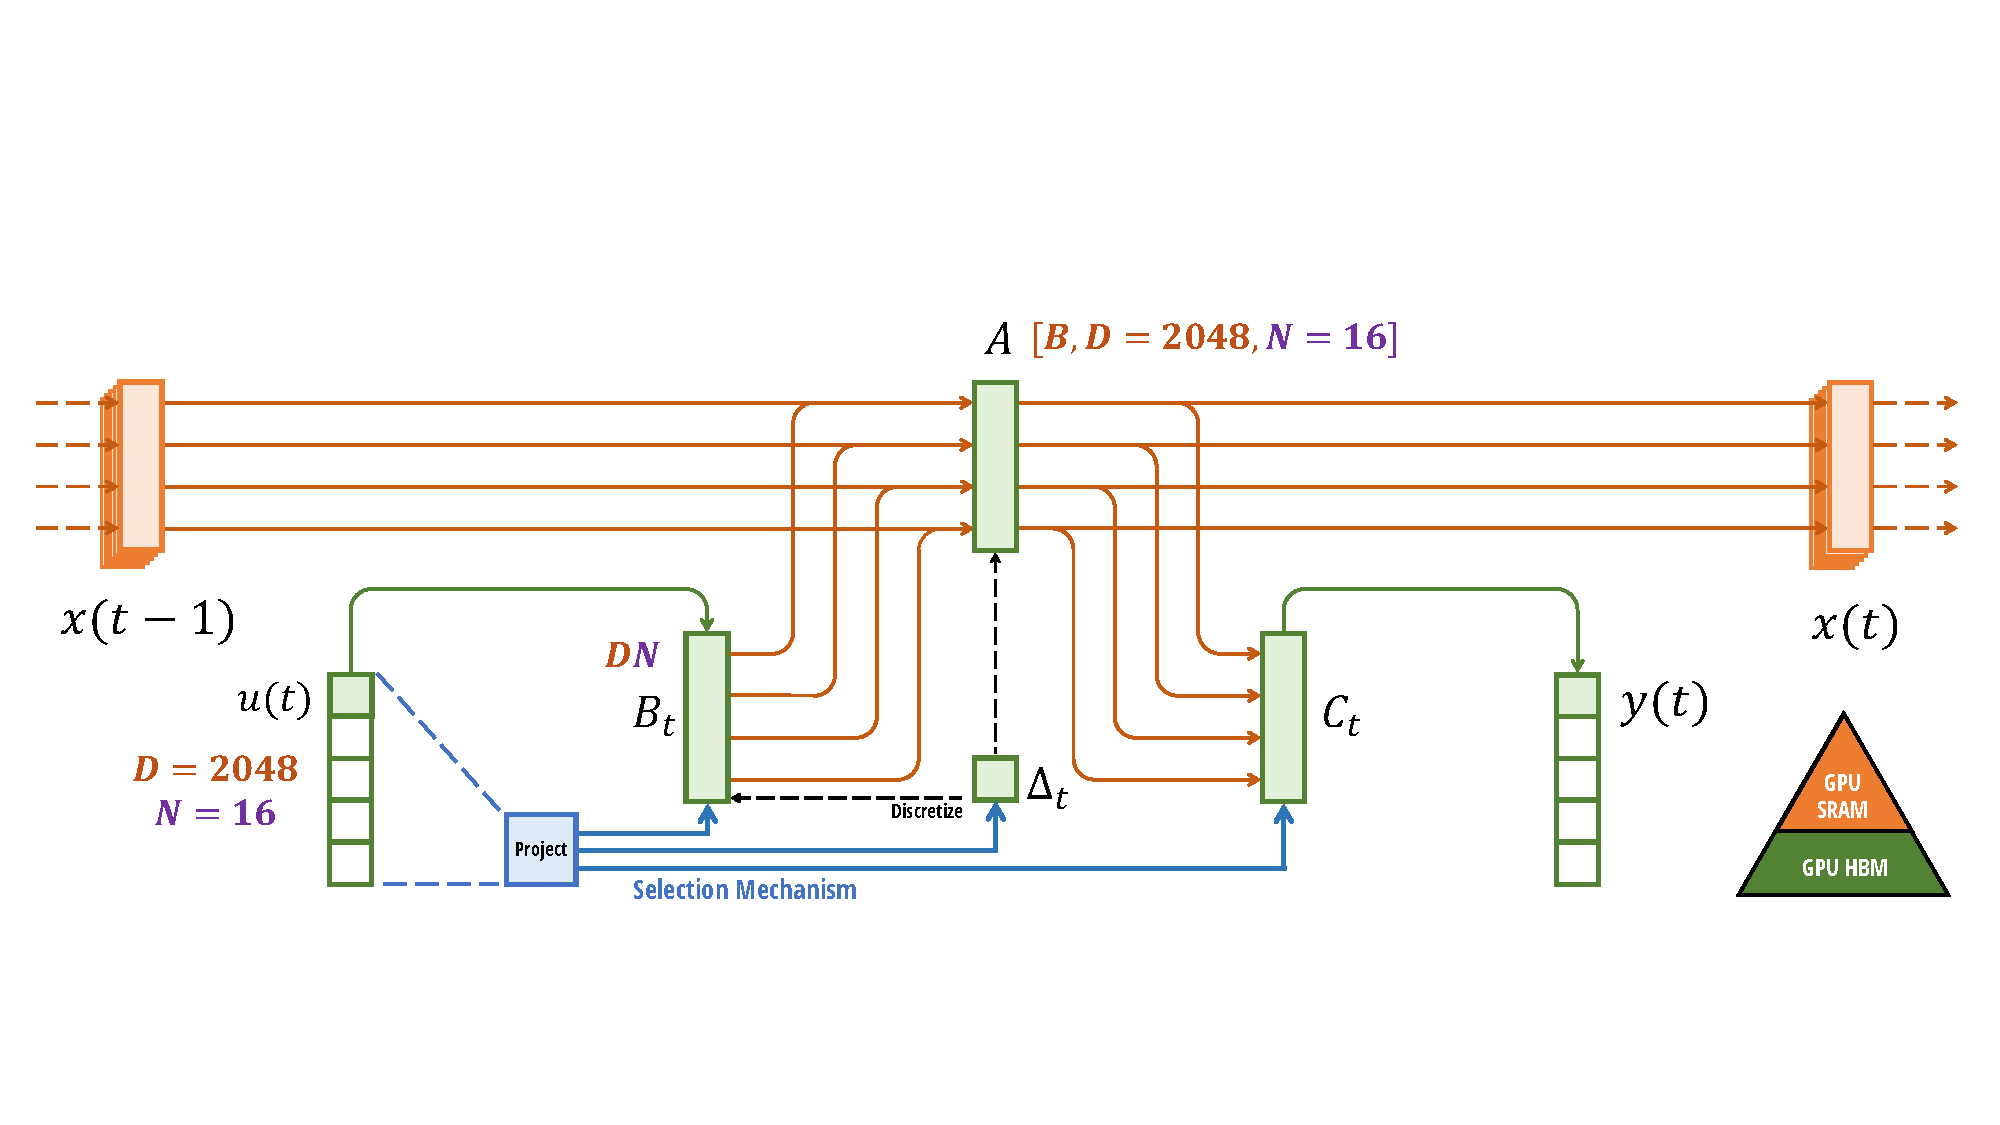
\includegraphics[width=0.9\textwidth]{figures/mamba-ssm.pdf}
  \caption{图\ref{fig:mamba-mixer}中SSM模块的细节}\label{fig:mamba-ssm}
\end{figure}

SSM内部带有隐状态$x(t)$,式\eqref{eq:ssm-0}通过隐状态$x(t)$把输入$u(t)$映射到$y(t)$。
一个离散化之后的SSM模型其可学习为:
\textcolor{red}{$\triangle$,$\mathbf{A}$,$\mathbf{B}$,$\mathbf{C}$,
$\mathbf{D}$}。
mamba中,$\mathbf{A}$和$\mathbf{D}$不依赖于输入;
$\mathbf{\triangle}$,$\mathbf{B}$和$\mathbf{C}$依赖于输入。

Listing \ref{ssm-code}中红色高亮的变量直接对应图\ref{fig:mamba-mixer}中右表中的可学习参数。

\begin{lstlisting}[language=cplus, caption={ssm in mamba},label={parallel-scan-mamba}, label={ssm-code}]
function SSM((:$u_{[B, L, 2048]}$:))(:$\rightarrow y(t)_{[B,L,2048]}$:)
  (:$v_0 = u(t)\ @ \ \textcolor{red}{\text{x\_proj}}^T$:)  // (:\textcolor{grey}{$[B,L,2048]@[2048,96]\rightarrow [B,L,96]$}:)
  (:$v_1, \mathbf{B}, \mathbf{C} = \text{split}(v_0)$:)  // (:\textcolor{grey}{$[B,L,64], [B,L,16], [B,L,16]$}:)
  (:$\triangle = \text{softplus}(v_1@\textcolor{red}{\text{delta\_proj}}^T + \textcolor{red}{\text{delta\_proj.bias}})$:) // (:\textcolor{grey}{$[B,L,64]@[2048,64]+[2048]\rightarrow [B,L,2048]$}:)
  (:$\bar{\mathbf{A}}=\exp\left(\triangle \textcolor{red}{\mathbf{A}}\right)$:)  // (:\textcolor{grey}{$[B,L,2048]@[2048,16]\rightarrow [B,L,2048,16]$}:)
  (:$\bar{\mathbf{V}}=\triangle\mathbf{B}u(t)$:) // (:\textcolor{grey}{$[B,L,2048]@[B,L,16]@[B,L,2048]\rightarrow [B,L,2048,16]$}:)

  // 9~12行是mamba代码中的selective_scan kernel
  (:$x(t)$:) = zeros((:$[B,2048,16]$:))  // scan的状态
  for (:$i$:) in (:$[0, L)$:):  // 把这个for循环实现成parallel scan
    (:$x(t) = \bar{\mathbf{A}}[:,i] * x(t) +\bar{\mathbf{V}}[:,i]$:)  // (:\textcolor{grey}{$[B, 2048, 16]$}:)
    (:$y(t)[:,i] = x(t) @ C[:,i]$:)  // bmm, (:\textcolor{grey}{$[B, 2048, 16]@[B,16]\rightarrow [B, 2048]$}:)
  (:$y(t) = y(t) + \textcolor{red}{\mathbf{D}}*u(t)$:)  // (:\textcolor{grey}{$[B, L, 2048]$}:)
\end{lstlisting}

% 其中$u(t)$的大小$[B, L, 2048]$, $A$大小$[2048,16]$,$D = 2048$,$A$和$D$是输入无关的,$\triangle$,$B$,$C$是input-dependent的(selective的)。

% \begin{enumerate}
% \item $v_0 = u(t) @ \textcolor{red}{W_1}$,$u(t)$是整个序列
% \item $v_1$, $B$, $C$ = $\text{split}(v_0)$,$v_1$用来计算$\triangle$,可以看到是输入相关的
% \item $\triangle = \text{softplus}(v_1 @ \textcolor{red}{W_2})$,这里$W_2$的大小是$[64,2048]$
% \item $y = \text{selective\_scan}(u(t), \triangle, A, B, C, D)$
% \end{enumerate}

% $W_1$的大小$[2048, 96]$,
% 这里的$96$是怎么来的呢?$96 = 64 + 16 * 2$。$64$是$\triangle$维度的大小,16是$B$和$C$的维度大小。
% 然后这个映射会被切分成$\triangle$,$B$和$C$

% $$y = \text{selective\_scan}(u, \triangle, \mathbf{A}, \mathbf{B}, \mathbf{C}, \mathbf{D})$$

% 上式中各个输入数据的大小:$u:[B, L, 2048]$,$\triangle:[B, L, 2048]$,$A:[2048,16]$,$B:[B, L, 16]$,$C:[B, L, 16]$,$D:[2048]$。

Listing \ref{ssm-code} 中5至13行对应了离散化SSM的两组公式:

\begin{align}
\bar{\mathbf{A}} &= \exp(\triangle \mathbf{A}) & [B, L, 2048, 16] \label{eq:mamba1}\\
\bar{\mathbf{V}} &= \bar{\mathbf{B}}u(t) = \triangle \mathbf{B} u(t) & [B, L, 2048,16]\label{eq:mamba2}\\
x(t+1)&=\bar{\mathbf{A}}x(t) + \bar{\mathbf{V}} & [B, 2048, 16]\label{eq:mamba3}\\
\textcolor{red}{y(t)} &\textcolor{red}{=\mathbf{C}x(t) + \mathbf{D}u(t)} & [B, L, 2048]\label{eq:mamba4}
\end{align}

$\eqref{eq:mamba1}$是ZOH离散化;$\eqref{eq:mamba2}$中,$\bar{\mathbf{B}} = \triangle \mathbf{B}$ 是简化的欧拉离散化(关于$A$和$B$离散化方法为什么这样选择,
参考\href{https://github.com/johnma2006/mamba-minimal/blob/master/model.py#L305}{这个项目}给出的一些说明。)
我们来看式\eqref{eq:mamba3}和\eqref{eq:mamba4}的实现。\textcolor{red}{公式\eqref{eq:mamba3}的实现就是一直存在诸多迷思的parallel scan}。

在Mamba之前的SSM都是对一个线性时不变系统进行模拟,由于在时间维度上没有依赖,训练时可以当做卷积进行计算。

图\ref{fig:ssm-overview}中$u(t)$是输入信号,是一个标量,$\vec{x}$是系统的状态,是一个向量。
$\mathbf{A}$,$\mathbf{B}$,$\mathbf{C}$是矩阵,形状如图所示,是作用于scalar输入信号的$u(t)$的SSM模型的参数。
$\mathbf{A}$矩阵是对角矩阵。因此,一个SSM模型的参数可以用$N$个数表示。

\begin{figure}[h]
  \centering
  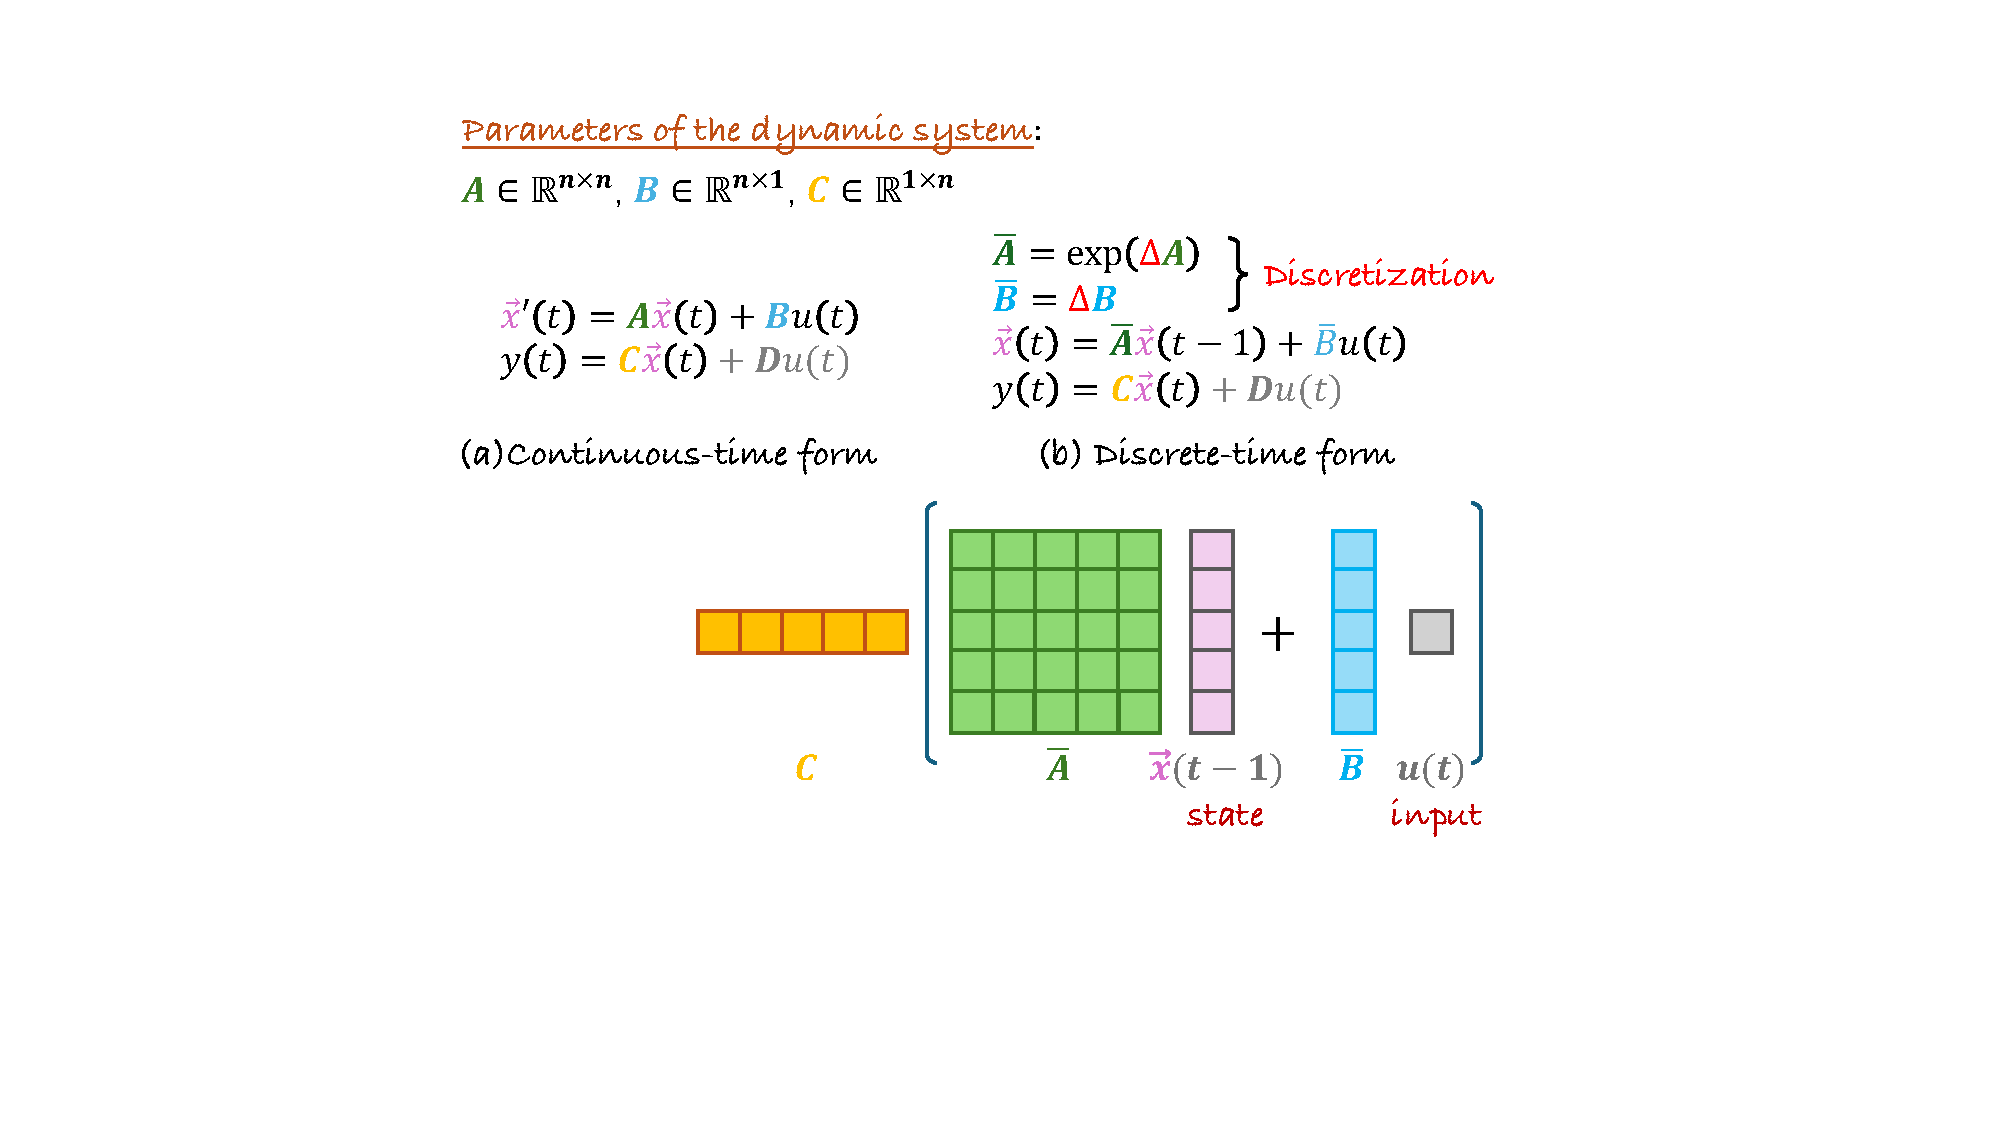
\includegraphics[width=0.6\textwidth]{figures/SSM-overview.pdf}
  \caption{作用于一个scalar input $u(t)$的SSM model,$\vec{x}$是状态}\label{fig:ssm-overview}
\end{figure}

机器学习任务中输入都是向量形式,假设为$D$。将图\ref{fig:ssm-overview}这样一个模型应用到向量输入的方法也非常直接:
引入$D$个独立的SSM模型,每个独立地作用于输入信号的一个维度。
假设输入序列的batch大小为:$B$,序列长度$L$,channel大小为$D$ (hidden size大小)。
于是,一个处理向量输入的SSM模型的有$DN$个参数。
处理完整个序列的时间和空间复杂度是:$O(BLDN)$,mamba的贡献之一是通过模型设计,解决这个时间和空间的复杂度。

% 使用data-dependent的gating进行decay,能够进一步改善学习效果。然后推导出这个gating机制的并行形式。